\documentclass[11pt]{beamer}
%%  ==========================================================================================  %%
%%                                              PAQUETES                                        %%
%%  ==========================================================================================  %%
\usepackage[utf8]{inputenc}
\usepackage[T1]{fontenc}
\usepackage[spanish, es-tabla]{babel}
\usepackage{amsmath}
\usepackage{amsfonts}
\usepackage{amssymb}
\usepackage{graphicx}
\usepackage{latexsym}
\usepackage{cancel}
\usepackage{float}
\usepackage{pst-knot}
\usepackage{epstopdf}
\usepackage{xcolor}
%%  ==========================================================================================  %%
%%                                        TEMA DE BEAMER                                        %%
%%  ==========================================================================================  %%
\usetheme{Warsaw} % tema de beamer
%%  ==========================================================================================  %%
%%                                           TÍTULO                                             %%
%%  ==========================================================================================  %%
\title{Ingeniería en Software II}
\subtitle[TPN1]{Trabajo Práctico N$^{\circ}$1\\ 
	Casos de investigación para desarrollar en clase}
\author{Ferreira, Juan D.\\ % Primer Autor
	    Viera, Ivan A.      % Segundo Autor
}
\titlegraphic{
\includegraphics[width=.75cm]{LogoIPF.eps}} % Logo del Instituto
%%  ====================================   DOCUMENTO    ======================================  %%
\begin{document}
	
	\begin{frame} % título
		\titlepage
	\end{frame}

	\begin{frame}
		\frametitle{Contenidos}
		\tableofcontents[pausesections]
	\end{frame}

	\section[Casos de fracaso]{Casos de fracaso}
	\begin{frame}
		\frametitle{Consignas}
		\begin{exampleblock}{Casos de fracaso}
			\begin{itemize}
				\item Establecer al menos 2 casos de fracaso en ingeniería de software.
				\item Describir los casos seleccionados.
				\item De ser posible especificar los motivos del abandono del proyecto y en que etapas se produjeron
				las fallas.
			\end{itemize}
		\end{exampleblock}
	\end{frame}

	\begin{frame}
		\frametitle{Caso 1: Expediente Virtual}
		\begin{block}{¿De qué se trata?}
			\begin{itemize}
				\item \textbf{Expediente Virtual} (o \textbf{FVC}) era un software de aplicación desarrollado por la FBI entre $2000$ y $2005$.
				\item El proyecto fue abandonado oficialmente en enero de $2005$, cuando aún estaba en fase de desarrollo y le costó al gobierno federal cerca de $\$170$ millones.
			\end{itemize}
		\end{block}
	\end{frame}

	\begin{frame}
		\frametitle{Caso 1: Expediente Virtual}
		\begin{block}{Las razones del fracaso:}
			\begin{itemize}
				\item El proyecto demostró un fracaso sistemático de la ingeniería de software prácticas.
				\pause
				\item La falta de un plan, desde el principio, llevó a las malas decisiones de arquitectura.
				\pause
				\item Los repetidos cambios en las especificaciones.
				\pause
				\item Microgestión de los desarrolladores de software.
				\pause
				\item La inclusión de gran parte del personal del FBI que tenía poco entrenamiento formal o no en la ciencia de la computación como gerentes e incluso los ingenieros en el proyecto.
				\pause
				\item Código abrumador debido a las especificaciones cambiantes y la exageración del alcance (El software tenía más de 700.000 líneas de código).
			\end{itemize}
		\end{block}
	\end{frame}

	\begin{frame}
		\frametitle{Caso 1: Expediente Virtual}
		\begin{block}{Consecuencias:}
			\begin{itemize}
				\item Fuertes críticas sociales tras el fracaso del programa VCF.
				\item Gran perdida de tiempo y dinero.
				\item La utilización del anticuado sistema de ACS, que muchos analistas sienten que está obstaculizando la oficina en la lucha contra el terrorismo.
			\end{itemize}
		\end{block}
	\end{frame}

	\begin{frame}
		\frametitle{Caso 2: National Institute of Standarts and Technology}
		\begin{block}{¿De qué se trata?}
			El Instituto Nacional de Normas y Tecnología(\textbf{NIST} por sus siglas en inglés, National Institute of Standards and Technology) es una agencia de la Administración de Tecnología del Departamento de Comercio de los Estados Unidos.
		\end{block}
	    \pause
	    \begin{block}{Mision}
	    	Es promover la innovación y la competencia industrial en Estados Unidos mediante avances en metrología, normas y tecnología para la cual tenia un software \textbf{NIST}, entre otras cosas.
	    \end{block}
	\end{frame}

	\begin{frame}
		\frametitle{Caso 2: National Institute of Standarts and Technology}
		\begin{figure}
			\centering
			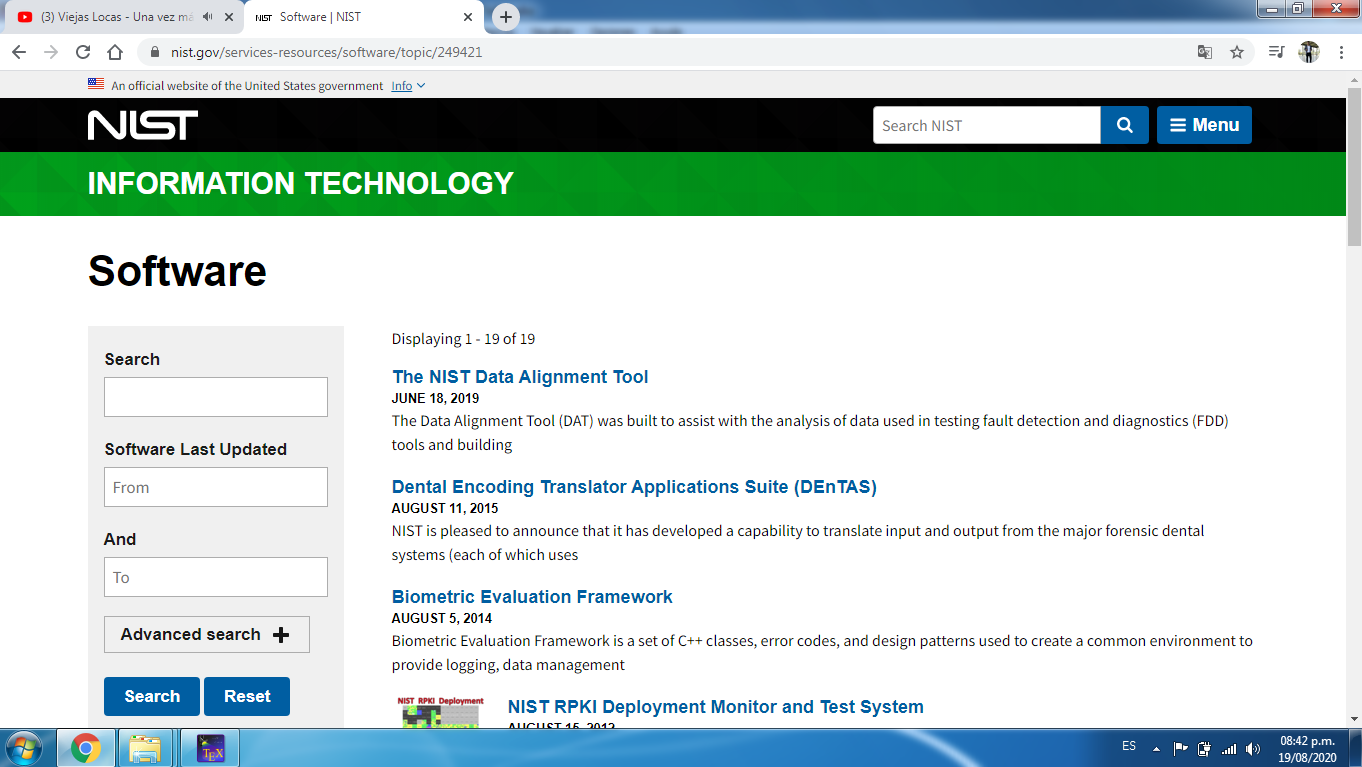
\includegraphics[width=\textheight]{NIST.PNG}
			\caption{{\scriptsize \url{https://www.nist.gov/services-resources/software/topic/249421}}}
		\end{figure}
	\end{frame}
    
    \begin{frame}
    	\frametitle{Caso 2: National Institute of Standarts and Technology}
    	\begin{block}{Razones del fracaso}
    		 Los errores de software, o errores, son tan frecuentes y perjudiciales. Según cálculos del \textit{Instituto Nacional de Estándares y Tecnología} (NIST) de los  estados Unidos, en el año $2002$ las pérdidas por errores del software en el mercado Norteamericano rondaron los $67,5$ mil millones de euros.
    		
    		\textbf{A nivel nacional, más de la mitad de los gastos son sufragados por los usuarios de software y el resto por los desarrolladores de software o vendedores}.
    	\end{block}
    \end{frame}

    \section{Casos De Éxitos}
    
    \begin{frame}
    	\frametitle{Consigna}
    	\begin{exampleblock}{Casos de Éxito}
    		\begin{itemize}
    			\item Establecer al menos 2 casos conocidos.
    			\item Enumerar sus beneficios respecto a los objetivos planteados
    			\item ¿Se ajustan los resultados a los requerimientos planteados?
    		\end{itemize}
    	\end{exampleblock}
    \end{frame}
    
    \begin{frame}
    	\frametitle{Caso 3: SkyMeD}
    	\begin{block}{¿En qué consiste?}
    		\begin{itemize}
    			\item Consiste en un Sistema de Relevamiento, Monitoreo y Gestión digital de datos para Instituciones de Salud y entidades de control que llevan adelante el control de personas en Aislamiento Social Obligatorio (ASO), ante la presencia de COVID-19.
    			\item  El 29 de abril comenzaron la carga de datos y se aventuraron en elaborar un sistema de monitoreo similar para Defensa Civil que informa en tiempo real a cada hospital de la zona, las personas que deben ser ingresadas a aislamiento, lo cual permite iniciar los protocolos de forma urgente, sin perder tiempo.
    		\end{itemize}
    	\end{block}
    \end{frame}
   
    \begin{frame}
    	\frametitle{Caso 3: SkyMeD}
    	\begin{block}{Idea}
    		Cuando apareció la pandemia, les pareció una buena idea realizar una acción de Responsabilidad Social Empresaria para colaborar con la situación y se pusieron manos a la obra.
    	\end{block}
        \pause
    	\begin{block}{Razones de su éxito}
    		\begin{enumerate}
    			\item La aplicación permite que las entidades cuenten en tiempo real con información estratégica para activar sus protocolos en forma inmediata.
    			\pause
    			\item El desarrollo puede ser adaptado a múltiples propositos (incluso post pandemia ) al trabajo con otras enfermedades como Hanta Virus y Dengue, o de plagas como la Mosca de la fruta.
    		\end{enumerate}
    	\end{block}
    \end{frame}

    \begin{frame}
    	\frametitle{Caso 3: SkyMeD}
    	\begin{block}{¿Se ajustan los resultados a los requerimientos planteados?}
    		\begin{itemize}
    			\item El emprendimiento si se ajusta a los requerimientos planteados ya que está está siendo utilizado por diversas instituciones públicas de la zona, que están armando un sistema de relevamiento de familias en riesgo de inundación
    			\item Existe otro proyecto con la Universidad Nacional de la Patagonia San Juan Bosco de Comodoro Rivadavia para un desarrollo tecnológico para plagas.
    		\end{itemize}
    	\end{block}
    \end{frame}
    
    \begin{frame}
    	\frametitle{Caso 4: Tik Tok}
    	\begin{block}{Actualidad}
    		\begin{itemize}
    			\item \textbf{TikTok}, es una red social de origen chino que permite grabar, editar y compartir vídeos cortos, que pisa fuerte en la actualidad. visuales.
    			\item  Tuvo un antecesor llamado Vine (la aplicación de Twitter que cerró hace algunos años),
    			\item Posee la particularidad de permitir a sus usuarios compartir vídeos cortos e instantáneos, con diversos efectos de sonido y filtros.
    		\end{itemize}
    	\end{block}
    \end{frame}
    
    \begin{frame}
    	\frametitle{Caso 4: Tik Tok}
        \begin{block}{Razones de su éxito}
        	\begin{enumerate}
        		\item La app china que ha adoptado lo mejor de otras APPs, para fusionar sus puntos más fuertes, y colocarse entre las aplicaciones móviles más utilizadas, hoy en día.
        		\pause
        		\item La app permite crear vídeos musicales de efecto inmediato e instantáneo,
        		\pause
        		\item Los videos que se pueden compartir duran entre $15$ y $60$ segundos. 
        	\end{enumerate}
        \end{block}
    \end{frame}

    \begin{frame}
   	    \frametitle{Caso 4: Tik Tok}
   	    \begin{block}{¿Se ajustan los resultados a los requerimientos planteados?}
   	    	La aplicacón se ajusta a los requerimientos planteados y cada vez es más común ver también a las marcas creando contenidos para visualizar sus productos. Incluso, a organizaciones como la de las Naciones Unidas utilizando la plataforma para suscitar interés en temas realmente importantes, como la hambruna mundial o el calentamiento global, a través del impulso de retos como el $\#danceforchange.$
   	    \end{block}
    \end{frame}
    
    \section{Caso Actual}
    
    \begin{frame}
    	\frametitle{Consignas}
    	\begin{exampleblock}{Caso Actual}
    		\begin{itemize}
    			\item Smartmatic: Elecciones argentina 2019
    			\item Establecer cuales les parece que fueron los requerimientos.
    			\item ¿Se cumplieron los objetivos?
    		\end{itemize}
    	\end{exampleblock}
    \end{frame}

    \begin{frame}
    	\frametitle{Caso 5: Smartmatic - Elecciones Argentina 2019}
    	\begin{block}{Smartmatic: Elecciones Argentina 2019}
    		\textbf{Smartmatic} es una empresa multinacional especializada en soluciones tecnológicas para aumentar la transparencia y mejorar la integridad de las elecciones.
    	\end{block}
    
        \pause
        
        Esta compañía se encuentra organizada en tres áreas de negocios:
        
        \pause
        
        \begin{enumerate}
        	\item \textbf{Soluciones electorales}: voto electrónico, planificiación y despliegue de proyectos electorales,
        	\pause
        	\item \textbf{Gestión de identidad}: registro civil, censo electoral, proyectos de registro y autenticación biométrica de personas y
        	\pause
        	\item \textbf{Soluciones para ciudades inteligentes (smart cities)}: en sistemas inteligentes de transporte público y plataformas de seguridad ciudadana.
        \end{enumerate}
    \end{frame}

    \begin{frame}
    	\frametitle{Caso 5: Smartmatic - Elecciones Argentina 2019}
    	\begin{block}{Los objetivos y requerimientos.}
    		La empresa Smartmatic le vendió a nuestro país un software llamado \href{https://www.smartmatic.com/es/elecciones/elecciones-manuales/smarttally/}{\textcolor{red}{SmartTally}}, solución que tiene como \textbf{objetivo} la transmisión de datos desde las escuelas. Algunos de los \textbf{requerimientos} del sistema fueron
    		\pause
    		\begin{enumerate}
    			\item Permitir que los telegramas de cada escuelas sean enviados de Forma virtual: antes, los telegramas se mandaban por vía terrestre al Correo,
    			\pause
    			\item Permitir mayor seguridad, ya que las actas de escrutinio se firman digitalmente antes de ser transmitidas,
    			\pause
    			\item Las autoridades también pueden utilizar la aplicación SmartTally para obtener información acerca del avance del proceso durante la jornada electoral
    		\end{enumerate}
    	\end{block}	
    \end{frame}

    \begin{frame}
    	\frametitle{Caso 5: Smartmatic - Elecciones Argentina 2019}
    	\begin{block}{Desempeño del sistema.}
    		 Si bien la carga de datos se realizó sin inconvenientes, esos datos no se pudieron visualizar hasta las $22:30hs$, cuando ya había más del $30\%$ de votos escrutados en todos los distritos y el gobierno resolvió darlos a conocer. Fue por eso que no se cumplió con el objetivo de difundir los resultados con el $10\%$ de los telegramas transmitidos, tal como había establecido.
    	\end{block}
        \pause
        \begin{block}{¿Cúal fue el problema?.}
        	El problema de ejecución fue que los telegramas estaban en el sistema, pero no se podian están convirtir del formato TIFF a pdf, como para que los podamos visualizar y ésto pudo haberse evitado utilizando algún complemento que agilice la conversión de formato TIFF a pdf.
        \end{block}
    \end{frame}
 
\end{document}
